\section{Explainable AI (xAI)}

Explainable AI is a growing field that comes with the need of humans to understand, or trust the models used. There are two main ways to get this goal:

\begin{enumerate}
	\item Agnostic methods, that query the model (potentially an exponential number of times) and draw conclusions from the results (methods as SHAP, LIME)

	\item Interpretable models - models with an interpretable process that can be explored in order to obtain further insights. For example, linear regression is defined by its coefficients. Observing these coefficients reflect the effect of the input features. Markov Chains models, as HMM, model an inner process that could later be explored. Usually, there is a trade-off between the model's complexity and their interpretablity.In recent years, the state of the art models have grown far more complex, making them uninterpretable.

\end{enumerate}


in the context of generative models, xAI contribution might have two aspects - both explore the abilities of the model and the generation process.

\subsection{Attention Models}

The attention mechanism was initially introduced on a machine translation task \cite{7}. The idea was to give the model the ability to filter, by itself, solely the relevant parts of the input at any point in time. In the original paper, it was done by adding another layer to the recurrent network. After the forward backward passes, the model weights all time steps outputs while generating every word. This is called the additive attention scheme.


The idea developed with the emergence of the transformer model \cite{8} which uses the same key idea - give the model the ability to filter the relevant data needed to generate the output. This time, the authors use the "Scaled Dot-Product Attention", which can be implemented much more efficiently, and is able to capture a more complex dependencies in the data.

This is the same type of attention that will be used in the ScrabbleGAN model and will be elaborated on chapter 5.


\begin{figure}[h]
\centering
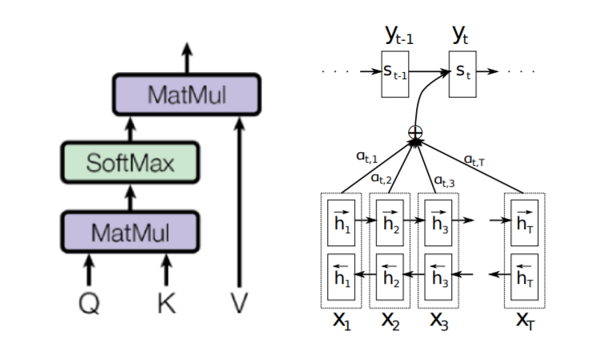
\includegraphics[scale=0.8]{attention_heads}
\caption{Right:Additive attention head Left:Scaled dot-product attention head}
\label{fig:x cubed graph}
\end{figure}


\begin{figure}[h]
\centering
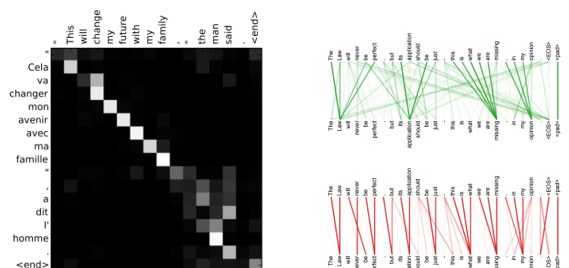
\includegraphics[scale=1]{attention_examples}
\caption{Example of features maps produced by exploring the attention mechanisms. Right: maps from additive attention in machine translation. Left: maps from two different scaled dot-product attention heads. Its clear hat parts of the input effects every output component.}
\label{fig:x cubed graph}
\end{figure}



\section{GAN models}

GAN model, first proposed in 2014 \cite{9}, is a generative model framework that consists of two networks that compete with each other - the Discriminator network tries to separate real images from fake ones, while the Generator network tries to generate real look-alike images.
GAN produces SOTA results in many fields, and it comes as no surprise that it has been adapted to solve many problems - from generating images (and its derivatives as super resolution tasks) to simulating complex physics systems.

\begin{figure}[h]
\centering
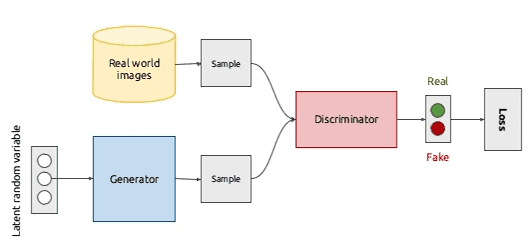
\includegraphics[scale=0.8]{GAN_scheme}
\caption{GAN model scheme \cite{12}}
\label{fig:x cubed graph}
\end{figure}

BiGAN is an extension of GAN, that adds another component to the classic GAN framework - Encoder. We train it to predict the random noise that was used to generate the image. 
The generator needs to maximize information that flows from the structure of the latent space to the image. We try to decode the latent space from the generated image, and by doing that we 'enforce' the generator to learn a better representation of the structure.
This process is supposed to make the latent space more interpretable - a meaningful representation means a successful encoder.

\begin{figure}[h]
\centering
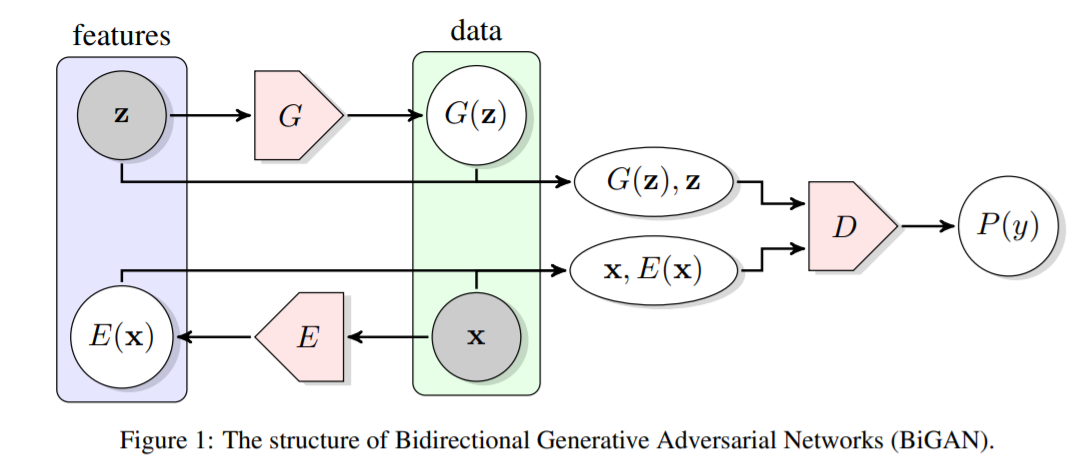
\includegraphics[scale=0.6]{bigan_scheme}
\caption{BiGAN model scheme \cite{12}}
\label{fig:x cubed graph}
\end{figure}


Another way to extract insights from the latent space is to enforce the latent space to a certain meaningful structure (as one with discrete structure).
InfoGAN \cite{12} is an example of merging these two ideas, which will be elaborated on chapter 5. 
Unsupervised Discovery of Interpretable Directions in the GAN Latent Space is also based on the same idea. This method is agnostic. The algorithm tries to find directions in the latent space that have meaningful effect in the output space.


\section{Generating Handwritten Text}

Handwriting generation is a relatively new field. It was first introduced by Graves \cite{3}, who synthesized online handwriting data (coordinates in 2D space) with RNN. Other works, as DeepWriting \cite{4} extended the same idea, adding more components to the model such as latent space sampling.

The output of these models is a list of probabilities. For each time step, the model generates the  distribution of the next point's coordinates.

The main contribution of Graves paper is the use of CTC - Connectionist Temporal Classification \cite{5} measurement as a loss function that can be used to train generative models. 

CTC measures the probability of text given the whole sequence generated. 
\centerline{$ P(Y|X) = \sum_{a\in A{X,Y}}\prod_{t=1}^{T}p_{t}(a_{t}|X) $} 
Y is the text, X is the image, and A is the group of all legal alignments between X and Y. 

The loss is alignment free, which means we don't need a segmented sequence as an input. Segmenting handwritten data is not trivial due to areas in the input data which don't belong to a single character. Therefore, finding a loss term that can deal with that characteristic of the data is crucial.

ScrabbleGAN \cite{6} is a handwriting generation model, that in contrast to Graves work, uses offline data (images of handwritten texts) instead of online data.
It also uses the same CTC loss technique, this time over slices of the image instead of coordinates.
